Organoids are "\textbf{mini organs}" built in the lab from stem cells.\\
Organoids \textbf{mimic geometric features} and \textbf{cell organization} of the original organ (tissue replica). The surrounding \textbf{ECM composition} is \textbf{custom} designed.\\

Matrigel: matrix scaffold for organoids, provides \textbf{mechanical support} and \textbf{adhesion sites} for cells.\\
Cell source: induced pluripotent SC (iPSC) terminally differentiated cells reprogrammed back to pluripotency.\\

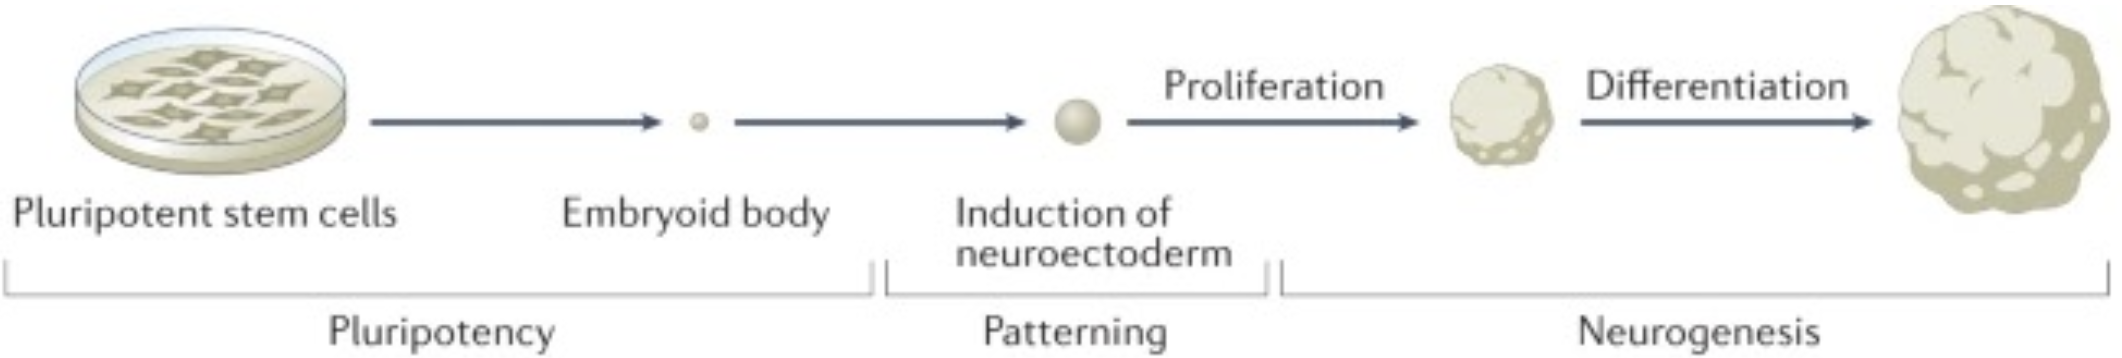
\includegraphics[width=40mm]{src/Images/organoid.png}


Possibility to \textbf{model genetic diseases} such as Parkinson in cerebral organoids.

\textbf{Limited to small size}, nutrient and oxygen supply is limited by diffusion.\\